\documentclass[12pt, openany]{book}

% --- PREAMBLE ---
\usepackage[utf8]{inputenc}
\usepackage[english]{babel}
\usepackage{graphicx}
\usepackage{amsmath, amssymb, amsfonts, amsthm}
\usepackage{geometry}
\usepackage{stix}
\geometry{a4paper, margin=1in}
\usepackage[dvipsnames]{xcolor} % For colors like 'purple'
\usepackage{hyperref}

% --- HYPERREF SETUP ---
\hypersetup{
    colorlinks=true,
    linkcolor=purple,
    filecolor=magenta,      
    urlcolor=cyan,
    citecolor=purple,
    pdftitle={Notes on Physical Optics},
    pdfpagemode=FullScreen,
}


% --- MATHEMATICAL ENVIRONMENTS DEFINITION ---
\theoremstyle{definition}
\newtheorem{definition}{Definition}[section]
\theoremstyle{plain}
\newtheorem{theorem}[definition]{Theorem}
\newtheorem{proposition}[definition]{Proposition}
\newtheorem{lemma}[definition]{Lemma}
\newtheorem{corollary}[definition]{Corollary}
\theoremstyle{remark}
\newtheorem{remark}[definition]{Remark}

% --- CUSTOM COMMANDS FOR PHYSICS ---
\newcommand{\R}{\mathbb{R}}
\newcommand{\C}{\mathbb{C}}
\newcommand{\pdv}[2]{\frac{\partial #1}{\partial #2}} % Partial derivative
\newcommand{\ddv}[2]{\frac{d #1}{d #2}} % Total derivative
\newcommand{\vecbf}[1]{\mathbf{#1}} % Bold vector
\newcommand{\vecx}{\mathbb{x}}

\geometry{a4paper, margin=1in}

\begin{document}

% --- Start of Custom Title Page ---
\begin{titlepage}
    \centering
    \vspace*{2cm} % Space at the top
    
    {\Huge\bfseries Vibenotes on Geometrical Optics\par}
    
    \vspace{1cm}
    
    {\Large\itshape 1st Partial Exam\par}

    \begin{figure}[h]
        \centering
        
\includegraphics[width=0.15\linewidth]{ciencias.png}
        \label{fig:placeholder}
    \end{figure}
    \vspace{0.5cm}

    \begin{figure}[h]
        \centering
        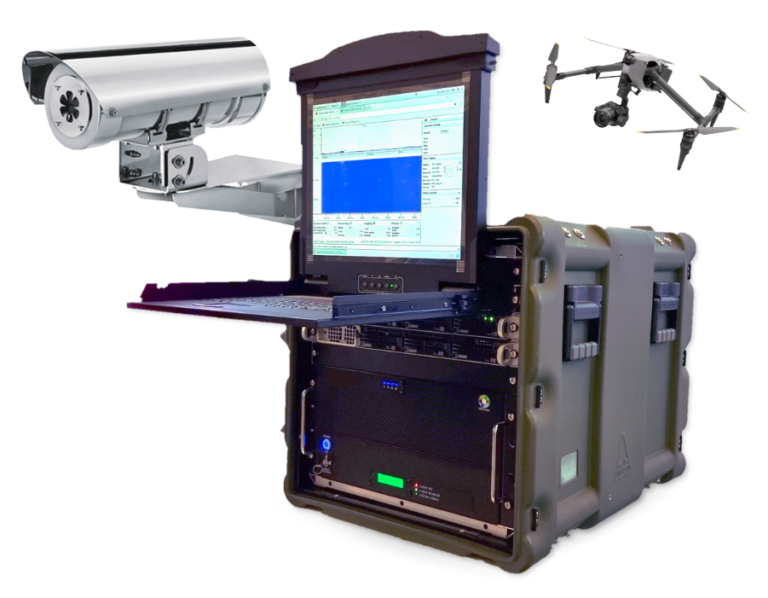
\includegraphics[width=0.85\linewidth]{optics.png}
        \caption{I have no fucking idea what this is but it looks cool as hell}
        \label{fig:placeholder}
    \end{figure} % Space between title and author
    
    
    {\large Based on "Geometrical Optics" by Hecht\par} \\
    \textit{By Andrés López}\\
    
    \vspace*{2cm} % Space at the bottom
\end{titlepage}
% --- End of Title Page ---

\newpage

This page is unintentionally left in blank.
\newpage

\tableofcontents

%\chapter{Geometrical Optics and Lenses}

\section{Fundamental Concepts}
\begin{itemize}
    \item \textbf{Geometrical Optics:} It is the study of light propagation in terms of rays, which travel in straight lines in homogeneous media. It is considered the limit where the wavelength tends to zero ($\lambda_0 \to 0$), ignoring effects such as diffraction and interference.
    \item \textbf{Point Source and Huygens' Principle:} A \textbf{point source} is an ideal emitter that radiates spherical waves. According to \textbf{Huygens' Principle}, any wavefront can be considered as a collection of countless point sources, where each emits its own spherical wavelets. The envelope of these wavelets forms the next wavefront.
    \item \textbf{Conjugate Points (S and P):} If rays originating from a point S converge to another point P after passing through an optical system, S and P are conjugate points. P is the \textbf{image} of S.
    \item \textbf{Real Image:} It is formed where light rays actually converge. It can be projected onto a screen.
    \item \textbf{Virtual Image:} It is formed where light rays appear to diverge. It cannot be projected onto a screen.
    \item \textbf{Optical Path Length (OPL):} In its generalized form, it is the integral of the refractive index along the path C: $OPL = \int_C n(s) ds$. For observation in a single homogeneous medium, it simplifies to $OPL = n \cdot d$. According to Fermat's Principle, light follows the path with the stationary OPL (minimum, maximum, or inflection).
\end{itemize}

\section{Refraction at Spherical Surfaces}

\begin{table}[h!]
\centering
\caption{Sign Convention for Spherical Refracting Surfaces and Thin Lenses (Light incident from the left)}
\begin{tabular}{ll}
\hline
\textbf{Quantity} & \textbf{Positive Sign (+)} \\ \hline
$s_o, f_o$ & to the left of V (vertex) \\
$x_o$ & to the left of $F_o$ (object focus) \\
$s_i, f_i$ & to the right of V (vertex) \\
$x_i$ & to the right of $F_i$ (image focus) \\
$R$ & if C (center of curvature) is to the right of V \\
$y_o, y_i$ & above the optical axis \\ \hline
\end{tabular}
\label{tab:signos_lentes}
\end{table}

\begin{table}[h!]
\centering
\caption{Meanings Associated with the Signs of Various Thin Lens and Spherical Interface Parameters}
\begin{tabular}{lcc}
\hline
\textbf{Quantity} & \multicolumn{1}{c}{\textbf{Sign (+) }} & \multicolumn{1}{c}{\textbf{Sign (-) }} \\ \hline
$s_o$ & Real object & Virtual object \\
$s_i$ & Real image & Virtual image \\
$f$ & Converging lens & Diverging lens \\
$y_o$ & Erect object & Inverted object \\
$y_i$ & Erect image & Inverted image \\
$M_T$ & Erect image & Inverted image \\ \hline
\end{tabular}
\label{tab:signos_significado}
\end{table}

In the paraxial approximation (rays close to the optical axis and with small angles), the relationship between the object distance ($s_o$) and the image distance ($s_i$) for a single spherical surface of radius $R$ separating two media with indices $n_1$ and $n_2$ is:

\begin{figure}[h]
    \centering
    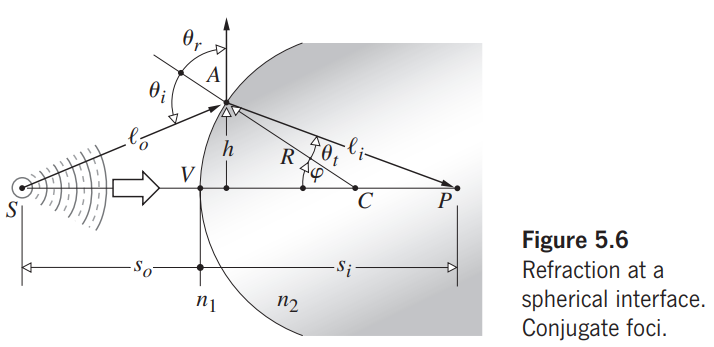
\includegraphics[width=0.7\linewidth]{1.png}
    \label{fig:placeholder}
\end{figure}

\vspace{0.5cm}
\noindent\fbox{%
\begin{minipage}{0.9\textwidth}
\begin{equation*}
    \frac{n_1}{s_o} + \frac{n_2}{s_i} = \frac{n_2 - n_1}{R}
\end{equation*}
\textbf{Hint:} This formula arises from applying Snell's Law in the paraxial approximation, where angles are small and we can use $\sin\theta \approx \theta$.
\end{minipage}
}
\vspace{0.5cm}

\begin{itemize}
    \item \textbf{Object Focal Length ($f_o$):} The object position for which the image is formed at infinity ($s_i = \infty$).
    $$ f_o = \frac{n_1 R}{n_2 - n_1} $$
    \item \textbf{Image Focal Length ($f_i$):} The image position when the object is at infinity ($s_o = \infty$).
    $$ f_i = \frac{n_2 R}{n_2 - n_1} $$
\end{itemize}

\section{Thin Lenses}
A thin lens is one whose thickness is negligible. Its behavior is described by two fundamental equations:

\begin{figure}[h]
    \centering
    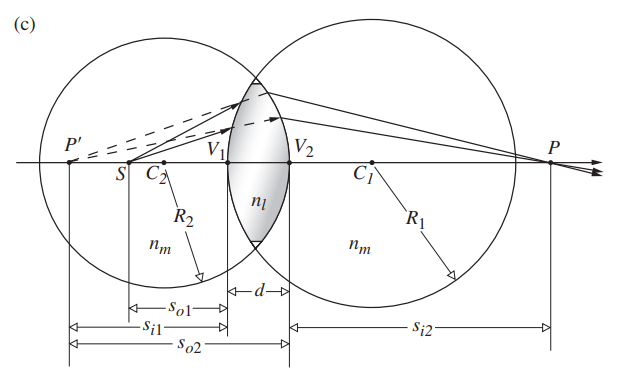
\includegraphics[width=0.55\linewidth]{spherical.png}
    \caption{A spherical lens}
    \label{fig:placeholder}
\end{figure}\\

\vspace{0.5cm}
\noindent\fbox{%
\begin{minipage}{0.9\textwidth}
\textbf{Lensmaker's Equation:} Relates the focal length ($f$) to the physical properties of the lens.
\begin{equation*}
    \frac{1}{f} = (n_l - 1) \left( \frac{1}{R_1} - \frac{1}{R_2} \right)
\end{equation*}
\textbf{Hint:} It is obtained by applying the refraction formula for a spherical surface to the two surfaces of the lens and assuming the thickness is zero.
\end{minipage}
}
\vspace{0.5cm}

\noindent\fbox{%
\begin{minipage}{0.9\textwidth}
\textbf{Gaussian Lens Equation:} Relates the positions of the object ($s_o$), the image ($s_i$), and the focus ($f$).
\begin{equation*}
    \frac{1}{s_o} + \frac{1}{s_i} = \frac{1}{f}
\end{equation*}
\textbf{Hint:} It is a simplification of the Lensmaker's Equation for practical use, note that it is a combination of the previous equations by applying transitivity.
\end{minipage}
}
\vspace{0.5cm}

\begin{itemize}
    \item \textbf{Converging Lenses (Positive):} They are thicker in the center. They have a positive focal length ($f > 0$) and converge parallel rays.
    \item \textbf{Diverging Lenses (Negative):} They are thinner in the center. They have a negative focal length ($f < 0$) and diverge parallel rays.
\end{itemize}

\vspace{1cm}

\subsubsection*{Images Formed by a Converging Lens (Convex)}
\begin{center}
\begin{tabular}{|l|llll|}
\hline
\multicolumn{1}{|c|}{\textbf{Object}} & \multicolumn{4}{c|}{\textbf{Image}} \\ \hline
\textbf{Position} & \textbf{Type} & \textbf{Position} & \textbf{Orientation} & \textbf{Relative Size} \\ \hline
$\infty > s_o > 2f$ & Real & $f < s_i < 2f$ & Inverted & Reduced \\
$s_o = 2f$ & Real & $s_i = 2f$ & Inverted & Same size \\
$f < s_o < 2f$ & Real & $\infty > s_i > 2f$ & Inverted & Magnified \\
$s_o = f$ & \multicolumn{4}{c|}{Image at $\pm \infty$} \\
$s_o < f$ & Virtual & $|s_i| > s_o$ & Erect & Magnified \\ \hline
\end{tabular}
\end{center}

\vspace{1cm}

\subsubsection*{Images Formed by a Diverging Lens (Concave)}
\begin{center}
\begin{tabular}{|l|llll|}
\hline
\multicolumn{1}{|c|}{\textbf{Object}} & \multicolumn{4}{c|}{\textbf{Image}} \\ \hline
\textbf{Position} & \textbf{Type} & \textbf{Position} & \textbf{Orientation} & \textbf{Relative Size} \\ \hline
Any position & Virtual & $|s_i| < |f|$, $s_o > |s_i|$ & Erect & Reduced \\ \hline
\end{tabular}
\end{center}

\section{Image Formation and Magnification}

\begin{figure}[h]
    \centering
    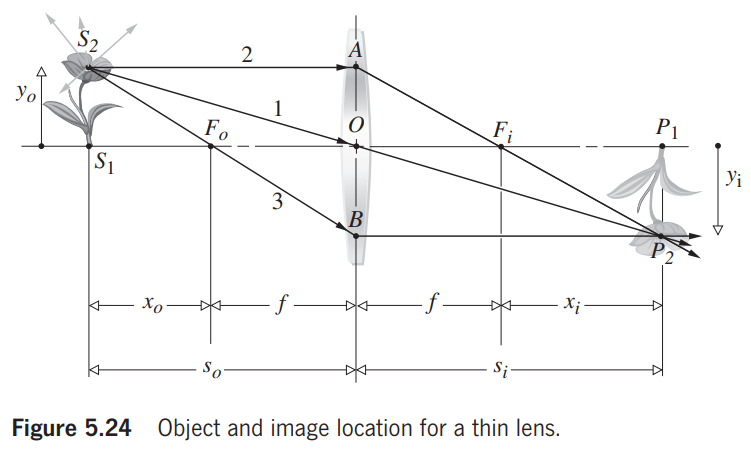
\includegraphics[width=0.75\linewidth]{diagram.png}
    \label{fig:placeholder}
\end{figure}

\begin{itemize}
    \item \textbf{Ray Tracing (Lenses):} The image of an object can be found graphically using three principal rays:
    \begin{enumerate}
        \item A ray passing through the optical center of the lens is not deviated.
        \item A ray parallel to the optical axis is refracted through the image focus ($F_i$).
        \item A ray passing through the object focus ($F_o$) is refracted parallel to the optical axis.
    \end{enumerate}
\end{itemize}

\noindent\fbox{%
\begin{minipage}{0.9\textwidth}
\textbf{Transverse Magnification ($M_T$):} It is the ratio of the image size ($y_i$) to the object size ($y_o$).
\begin{equation*}
    M_T = \frac{y_i}{y_o} = -\frac{s_i}{s_o}
\end{equation*}
\textbf{Hint:} It is derived from the similarity of triangles formed by the ray passing through the optical center. The negative sign indicates that a real image ($s_i > 0$) is inverted.
\end{minipage}
}
\vspace{0.5cm}

\noindent\fbox{%
\begin{minipage}{0.9\textwidth}
\textbf{Newtonian Formula:} Relates the distances from the foci.
\begin{equation*}
    x_o x_i = f^2
\end{equation*}
\textbf{Hint:} It is an alternative form of the Gaussian equation, useful when measuring from the foci instead of the lens center.
\end{minipage}
}

\section{Combination of Lenses}
The analysis of systems with multiple lenses is based on a simple principle: the image formed by the first lens becomes the \textbf{object} for the second lens, and so on. The image from the previous lens can be a real object (if it forms before the next lens) or a virtual object (if it would form after the next lens).

\subsection*{Lenses in Contact}
When two thin lenses are in contact ($d \to 0$), they behave as a single thin lens whose power is the sum of the individual powers.

\vspace{0.5cm}
\noindent\fbox{%
\begin{minipage}{0.9\textwidth}
\textbf{Effective Focal Length (Lenses in Contact):}
\begin{equation*}
    \frac{1}{f_{\text{eff}}} = \frac{1}{f_1} + \frac{1}{f_2}
\end{equation*}
\textbf{Hint:} This is the simplest form of combination. It is deduced by treating the image of $L_1$ as the object for $L_2$ and letting the separation $d$ tend to zero in the more general equations.
\end{minipage}
}
\vspace{0.5cm}

\subsection*{Separated Lenses}
When lenses are separated by a distance $d$, the system can no longer be described with a single focal length measured from a single point. Instead, two principal focal lengths are defined, measured from the outer lenses of the system.

\subsubsection*{Back Focal Length (b.f.l.)}
The \textbf{physical meaning} of the b.f.l. is that it indicates where the final focus will be formed for rays entering the system parallel (i.e., from an object at infinity). It is the distance from the vertex of the \textbf{last lens} to the image focal point of the entire system. It is crucial for knowing where to place a sensor or film.

\vspace{0.5cm}
\noindent\fbox{%
\begin{minipage}{0.9\textwidth}
\textbf{Back Focal Length Formula:}
\begin{equation*}
    \text{b.f.l.} = \frac{f_2(d - f_1)}{d - (f_1 + f_2)}
\end{equation*}
\textbf{Hint:} It is obtained by taking the limit as the initial object is at infinity ($s_{o1} \to \infty$) and calculating the position of the final image ($s_{i2}$) with respect to the second lens.
\end{minipage}
}
\vspace{0.5cm}

\subsubsection*{Front Focal Length (f.f.l.)}
The \textbf{physical meaning} of the f.f.l. is that it indicates where an object must be placed so that the rays exit the system parallel (i.e., so that the final image is at infinity). It is the distance from the vertex of the \textbf{first lens} to the object focal point of the entire system.

\vspace{0.5cm}
\noindent\fbox{%
\begin{minipage}{0.9\textwidth}
\textbf{Front Focal Length Formula:}
\begin{equation*}
    \text{f.f.l.} = \frac{f_1(d - f_2)}{d - (f_1 + f_2)}
\end{equation*}
\textbf{Hint:} It is obtained by imposing the condition that the final image is at infinity ($s_{i2} \to \infty$) and calculating the required position of the initial object ($s_{o1}$) with respect to the first lens.
\end{minipage}
}

\chapter{Stops and Mirrors}

\section{*Stops}
\begin{itemize}
    \item \textbf{Aperture Stop (A.S.):} The physical element that limits the amount of light reaching the image. It determines the brightness.
    \item \textbf{Field Stop (F.S.):} The element that limits the size of the object that can be seen. It determines the field of view.
    \item \textbf{Entrance Pupil:} The image of the A.S. as seen from the object space.
    \item \textbf{Exit Pupil:} The image of the A.S. as seen from the image space. This is where the eye should be placed.
\end{itemize}

\section{*Relative Aperture and f-number}
\noindent\fbox{%
\begin{minipage}{0.9\textwidth}
\textbf{f-number ($f/\#$):} Relates the focal length ($f$) and the diameter of the entrance pupil ($D$).
\begin{equation*}
    f/\# = \frac{f}{D}
\end{equation*}
\textbf{Hint:} It is a definition that relates the light-gathering capability (diameter D) with the magnification (focal length f). A small f-number implies a "fast" lens.
\end{minipage}
}

\section{Spherical Mirrors}
Unlike plane mirrors, spherical mirrors can focus light and form magnified or reduced images. They are governed by two fundamental equations in the paraxial approximation.

\begin{table}[h!]
\centering
\caption{Sign Convention for Spherical Mirrors}
\begin{tabular}{lcc}
\hline
\textbf{Quantity} & \multicolumn{1}{c}{\textbf{Sign (+) }} & \multicolumn{1}{c}{\textbf{Sign (-) }} \\ \hline
$s_o$ & Left of V, real object & Right of V, virtual object \\
$s_i$ & Left of V, real image & Right of V, virtual image \\
$f$ & Concave mirror & Convex mirror \\
$R$ & C to the right of V, convex & C to the left of V, concave \\
$y_o$ & Above axis, erect object & Below axis, inverted object \\
$y_i$ & Above axis, erect image & Below axis, inverted image \\ \hline
\end{tabular}
\label{tab:signos_espejos}
\end{table}

\vspace{0.5cm}
\noindent\fbox{%
\begin{minipage}{0.9\textwidth}
\textbf{Mirror Formula (in terms of R):} Relates the object ($s_o$) and image ($s_i$) distances with the radius of curvature ($R$) of the mirror.
\begin{equation*}
    \frac{1}{s_o} + \frac{1}{s_i} = -\frac{2}{R}
\end{equation*}
\textbf{Hint:} This is the main form of the equation, derived directly from the Law of Reflection and the geometry of triangles in the paraxial approximation.
\end{minipage}
}
\vspace{0.5cm}

\noindent\fbox{%
\begin{minipage}{0.9\textwidth}
\textbf{Focal Length ($f$):} It is defined in terms of the radius of curvature.
\begin{equation*}
    f = -\frac{R}{2}
\end{equation*}
\textbf{Hint:} For paraxial rays, the focus of a spherical mirror is located halfway to the center of curvature. The negative sign is a consequence of the sign convention (for a concave mirror, $R<0$, resulting in a positive focus, $f>0$).
\end{end{minipage}
}
\vspace{0.5cm}

By combining the two expressions above, we obtain the most common form of the mirror formula, which is identical to the thin lens equation:
$$ \frac{1}{s_o} + \frac{1}{s_i} = \frac{1}{f} $$

\begin{itemize}
    \item \textbf{Concave Mirrors:} They have $R < 0$, so their focal length is positive ($f > 0$). They behave analogously to converging lenses.
    \item \textbf{Convex Mirrors:} They have $R > 0$, so their focal length is negative ($f < 0$). They behave analogously to diverging lenses.
\end{itemize}

\subsection*{Image Characteristics for Spherical Mirrors}
The following table summarizes the properties of the image formed by concave and convex mirrors for a real object.

\vspace{0.5cm}
\subsubsection*{Concave Mirror}
\begin{center}
\begin{tabular}{|l|llll|}
\hline
\multicolumn{1}{|c|}{\textbf{Object}} & \multicolumn{4}{c|}{\textbf{Image}} \\ \hline
\textbf{Position} & \textbf{Type} & \textbf{Position} & \textbf{Orientation} & \textbf{Relative Size} \\ \hline
$\infty > s_o > 2f$ & Real & $f < s_i < 2f$ & Inverted & Reduced \\
$s_o = 2f$ & Real & $s_i = 2f$ & Inverted & Same size \\
$f < s_o < 2f$ & Real & $\infty > s_i > 2f$ & Inverted & Magnified \\
$s_o = f$ & \multicolumn{4}{c|}{Image at $\pm \infty$} \\
$s_o < f$ & Virtual & $|s_i| > s_o$ & Erect & Magnified \\ \hline
\end{tabular}
\end{center}

\vspace{1cm}

\subsubsection*{Convex Mirror}
\begin{center}
\begin{tabular}{|l|llll|}
\hline
\multicolumn{1}{|c|}{\textbf{Object}} & \multicolumn{4}{c|}{\textbf{Image}} \\ \hline
\textbf{Position} & \textbf{Type} & \textbf{Position} & \textbf{Orientation} & \textbf{Relative Size} \\ \hline
Any position & Virtual & $|s_i| < |f|$, $s_o > |s_i|$ & Erect & Reduced \\ \hline
\end{tabular}
\end{center}

\chapter{Prisms and Fiber Optics}

\section{Prisms}

\begin{itemize}
    \item \textbf{Dispersing Prisms:} They separate light by color due to the dependence of $n$ on $\lambda$.
\end{itemize}

\begin{figure}[h]
    \centering
    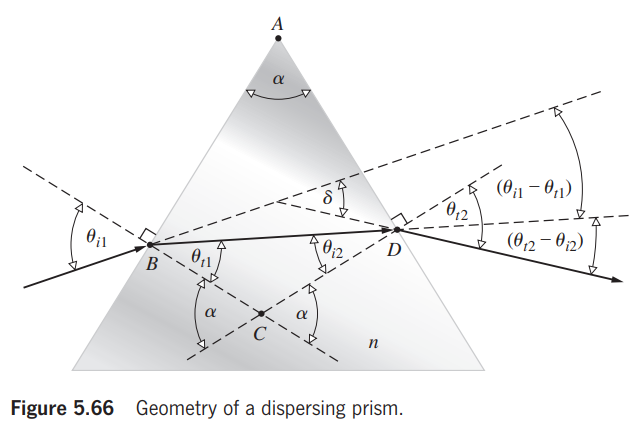
\includegraphics[width=0.55\linewidth]{prims disp.png}
    \label{fig:placeholder}
\end{figure}

\noindent\fbox{%
\begin{minipage}{0.9\textwidth}
\textbf{Refractive Index from Minimum Deviation ($\delta_m$):}
\begin{equation*}
    n = \frac{\sin\left(\frac{\delta_m + \alpha}{2}\right)}{\sin\left(\frac{\alpha}{2}\right)}
\end{equation*}
\textbf{Hint:} It is obtained by applying Snell's Law on both faces under the symmetric condition of minimum deviation, where the internal ray is parallel to the base.
\end{minipage}
}

\begin{itemize}
    \item \textbf{Reflecting Prisms:} They use total internal reflection to deviate light or invert images (e.g., Porro prism in binoculars).
\end{itemize}

\section{Fiber Optics}
They guide light through total internal reflection (TIR). They consist of a core ($n_f$) and a cladding ($n_c$), with $n_f > n_c$.

\noindent\fbox{%
\begin{minipage}{0.9\textwidth}
\textbf{Numerical Aperture (NA):} A measure of the fiber's ability to capture light.
\begin{equation*}
    \text{NA} = n_i \sin\theta_{\text{max}} = \sqrt{n_f^2 - n_c^2}
\end{equation*}
\textbf{Hint:} It comes from applying Snell's Law at the entrance face and the TIR condition ($ \sin\theta_c = n_c/n_f $) at the core-cladding interface.
\end{minipage}
}

\chapter{Optical Systems}
\section{The Human Eye and its Correction}
\begin{itemize}
    \item The eye forms a real and inverted image on the retina.
    \item \textbf{Myopia (Nearsightedness):} The eye is too convergent. It is corrected with a \textbf{diverging} (negative) lens.
    \item \textbf{Hyperopia (Farsightedness):} The eye is not convergent enough. It is corrected with a \textbf{converging} (positive) lens.
\end{itemize}

\noindent\fbox{%
\begin{minipage}{0.9\textwidth}
\textbf{Dioptric Power ($\mathcal{P}$):} The inverse of the focal length in meters.
\begin{equation*}
    \mathcal{P} \text{ [D]} = \frac{1}{f \text{ [m]}}
\end{equation*}
\textbf{Hint:} It is a definition of convenience. The power of lenses in contact adds up: $\mathcal{P} = \mathcal{P}_1 + \mathcal{P}_2$.
\end{minipage}
}

\section{Optical Instruments}
\noindent\fbox{%
\begin{minipage}{0.9\textwidth}
\textbf{Angular Magnification (Magnifier, image at $\infty$):}
\begin{equation*}
    MP = \frac{d_o}{f} \approx \frac{25 \text{ cm}}{f}
\end{equation*}
\textbf{Hint:} Compares the angle subtended by the virtual image with the angle subtended by the object at the near point ($d_o \approx 25$ cm).
\end{minipage}
}
\vspace{0.5cm}

\noindent\fbox{%
\begin{minipage}{0.9\textwidth}
\textbf{Angular Magnification (Microscope):}
\begin{equation*}
    MP = M_{To} M_{Ae} = \left(-\frac{L}{f_o}\right)\left(\frac{d_o}{f_e}\right)
\end{equation*}
\textbf{Hint:} It is the product of the linear magnification of the objective ($M_{To}$) and the angular magnification of the eyepiece ($M_{Ae}$). $L$ is the tube length ($\approx 160$ mm).
\end{minipage}
}
\vspace{0.5cm}

\noindent\fbox{%
\begin{minipage}{0.9\textwidth}
\textbf{Angular Magnification (Microscope):}
\begin{equation*}
    MP = M_{To} M_{Ae} = \left(-\frac{L}{f_o}\right)\left(\frac{d_o}{f_e}\right)
\end{equation*}
\textbf{Hint:} It is the product of the linear magnification of the objective ($M_{To}$) and the angular magnification of the eyepiece ($M_{Ae}$). $L$ is the tube length ($\approx 160$ mm).
\end{minipage}
}
\vspace{0.5cm}

\noindent\fbox{%
\begin{minipage}{0.9\textwidth}
\textbf{Angular Magnification (Telescope):}
\begin{equation*}
    MP = -\frac{f_o}{f_e}
\end{equation*}
\textbf{Hint:} It is the ratio of the subtended angles, which by similarity of triangles becomes the ratio of the focal lengths of the objective and the eyepiece.
\end{minipage}
}

\chapter{Thick Lenses}
Unlike a thin lens, a \textbf{thick lens} is one whose thickness is not negligible. To analyze these systems accurately, \textbf{analytical ray tracing} and its elegant formulation, the \textbf{matrix method}, are used.

\section{The Transfer Matrix Method}
The central idea is to model the path of a paraxial ray through an optical system using matrix operations. Each ray is represented by a vector and each element or space in the system by a matrix.

\begin{enumerate}
    \item \textbf{Ray Vector ($r$):} Describes the state of a ray by its height ($y$) and its weighted angle ($n\alpha$) at a point on the axis.
    \item \textbf{Operation Matrices:} They are applied to the ray vector to transform it. The two basic operations are:
    \begin{itemize}
        \item \textbf{Refraction ($\mathfrak{R}$):} The change in the ray's direction at an interface.
        \item \textbf{Translation ($\mathfrak{T}$):} The straight-line advance of the ray through a medium.
    \end{itemize}
\end{enumerate}

\vspace{0.5cm}
\noindent\fbox{%
\begin{minipage}{0.9\textwidth}
\textbf{Ray Vector ($r$):} Describes the height ($y$) and angle ($\alpha$) of a ray at a given point.
\begin{equation*}
    r = \begin{bmatrix} n\alpha \\ y \end{bmatrix}
\end{equation*}
\textbf{Hint:} This vector contains all the necessary information for a paraxial ray. The weighted angle ($n\alpha$) is used because it is modified simply in refraction and is conserved in translation.
\end{minipage}
}
\vspace{0.5cm}

\noindent\fbox{%
\begin{minipage}{0.9\textwidth}
\textbf{Refraction Matrix ($\mathfrak{R}$):} Models the change in the ray's direction as it passes through a surface of power $\mathcal{D}$.
\begin{equation*}
    \mathfrak{R} = \begin{bmatrix} 1 & -\mathcal{D} \\ 0 & 1 \end{bmatrix} \quad \text{where} \quad \mathcal{D} = \frac{n_t - n_i}{R}
\end{equation*}
\textbf{Hint:} This matrix only affects the ray's angle ($n\alpha$), not its height. The element $-\mathcal{D}$ represents the "strength" of the surface to bend light.
\end{minipage}
}
\vspace{0.5cm}

\noindent\fbox{%
\begin{minipage}{0.9\textwidth}
\textbf{Translation Matrix ($\mathfrak{T}$):} Models the straight-line travel of the ray over a distance $d$ in a medium of index $n$.
\begin{equation*}
    \mathfrak{T} = \begin{bmatrix} 1 & 0 \\ d/n & 1 \end{bmatrix}
\end{equation*}
\textbf{Hint:} This matrix only affects the ray's height ($y$), not its angle. The term $d/n$ represents the change in height due to propagation.
\end{minipage}
}
\vspace{0.5cm}

\section{The System Matrix and Cardinal Points}
To obtain the total effect of a thick lens, the matrices for each operation are multiplied in the \textbf{reverse} order to which the light encounters them. For a lens of thickness $d_l$ and index $n_l$:
$$ \mathcal{A} = \mathfrak{R}_2 \mathfrak{T}_{21} \mathfrak{R}_1 $$
This \textbf{System Matrix ($\mathcal{A}$)} encapsulates all the properties of the lens. Most powerfully, its elements are directly related to the \textbf{cardinal points}, which are the reference points that define any optical system.

\vspace{0.5cm}
\noindent\fbox{%
\begin{minipage}{0.9\textwidth}
\textbf{System Matrix ($\mathcal{A}$) for a Thick Lens:}
\begin{equation*}
\mathcal{A} = \begin{bmatrix} 1-\frac{\mathcal{D}_2 d_l}{n_l} & -\mathcal{D}_1-\mathcal{D}_2+\frac{\mathcal{D}_1 \mathcal{D}_2 d_l}{n_l} \\ \frac{d_l}{n_l} & 1-\frac{\mathcal{D}_1 d_l}{n_l} \end{bmatrix} = \begin{bmatrix} a_{11} & a_{12} \\ a_{21} & a_{22} \end{bmatrix}
\end{equation*}
\textbf{Hint:} The determinant of this matrix is always 1 ($|\mathcal{A}|=1$).
\end{minipage}
}
\vspace{0.5cm}

The cardinal points (focal points, principal planes, and nodal points) can be calculated directly from the elements of $\mathcal{A}$.

\begin{figure}[h]
    \centering
    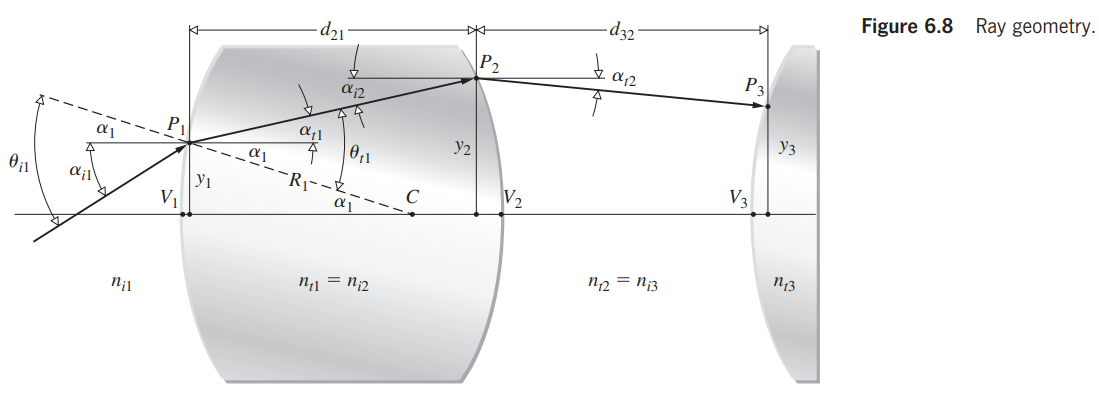
\includegraphics[width=0.85\linewidth]{rayt.png}
    \caption{Cardinal points and ray tracing in a thick lens.}
    \label{fig:placeholder}
\end{figure}

\begin{itemize}
    \item \textbf{Focal Points ($F_o, F_i$):} Define where rays focus or appear to originate from.
    \item \textbf{Principal Planes ($H_1, H_2$):} Are the theoretical planes where all refraction occurs. The focal length is measured from them.
    \item \textbf{Nodal Points ($N_1, N_2$):} A ray directed at $N_1$ emerges from $N_2$ with the same direction. In air, they coincide with the principal planes.
\end{itemize}

\noindent\fbox{%
\begin{minipage}{0.9\textwidth}
\textbf{Effective Focal Length ($f$):} The total power of the lens ($1/f$) is contained in the element $a_{12}$.
\begin{equation*}
    \frac{1}{f} = -a_{12}
\end{equation*}
\textbf{Hint:} This element represents the converging/diverging capability of the entire system.
\end{minipage}
}
\vspace{0.5cm}

\noindent\fbox{%
\begin{minipage}{0.9\textwidth}
\textbf{Position of the Principal Planes ($h_1, h_2$):} They are calculated from the lens vertices ($V_1, V_2$).
\begin{align*}
    h_1 &= \overline{V_1 H_1} = \frac{1-a_{11}}{-a_{12}} \\
    h_2 &= \overline{V_2 H_2} = \frac{a_{22}-1}{-a_{12}}
\end{align*}
\textbf{Hint:} These formulas locate the theoretical planes of refraction. A positive value means the plane is to the right of the vertex.
\end{minipage}
}
\vspace{0.5cm}

\section{Using Thick Lenses: Equations and Ray Tracing}
Once the effective focal length ($f$) and the position of the principal planes ($H_1, H_2$) are known, the analysis of a thick lens becomes very similar to that of a thin lens.

\begin{itemize}
    \item \textbf{Graphical Ray Tracing:} The same three principal rays are used, but refraction occurs at the planes $H_1$ and $H_2$, not at the center of the lens.
    \item \textbf{Lens Equations:} The Gaussian and Newtonian formulas are valid if the distances are measured from the principal planes.
\end{itemize}

\noindent\fbox{%
\begin{minipage}{0.9\textwidth}
\textbf{Gaussian and Newtonian Equations:}
\begin{align*}
    \frac{1}{s_o} + \frac{1}{s_i} &= \frac{1}{f} \\
    x_o x_i &= f^2
\end{align*}
\textbf{Hint:} The classic formulas work! The key is to measure $s_o$ and $x_o$ from the first principal plane ($H_1$), and $s_i$ and $x_i$ from the second principal plane ($H_2$).
\end{minipage}
}
\chapter{The Propagation of Light: A Wave Formalism}

\section{The Differential Wave Equation: A Unified Description}

In the pantheon of physics, few equations command such a wide dominion as the differential wave equation. It is the unifying principle that governs phenomena as disparate as the ripples on a pond, the vibrations of a violin string, the propagation of sound, and, most profoundly for our purposes, the flight of light itself.

\begin{theorem}[The Differential Wave Equation]
A physical disturbance, described by a scalar or vector function $\psi(\vecx, t)$, constitutes a wave if it is a solution to the linear, second-order, homogeneous partial differential equation:
$$ \nabla^2 \psi(\vecx, t) = \frac{1}{v^2} \frac{\partial^2 \psi(\vecx, t)}{\partial t^2} : \nabla^2 \equiv \sum_{i=1}^{3} \frac{\partial^2}{\partial x_i^2} $$
The constant $v$, with units of velocity, is a characteristic of the medium of propagation. The operator $\nabla^2$ quantifies how the value of $\psi$ at a point deviates from the average value in its immediate neighborhood. It is the spatial analogue of the second derivative.
\end{theorem}

\subsection{Mathematical Properties and Physical Interpretation}
The austere form of the wave equation belies a deep physical intuition encoded in its mathematical structure.

\begin{proposition}[Analysis of Properties]
The wave equation's form is a direct consequence of fundamental physical principles:
\begin{enumerate}
    \item \textbf{Linearity and Superposition:} The equation is \textbf{linear} because $\psi$ and its derivatives appear only to the first power. This is not merely a mathematical convenience; it is the formal statement of the \textbf{Principle of Superposition}. It asserts that, in a linear medium, wave amplitudes add together, allowing waves to pass through one another unaltered. If the wave equation were nonlinear, two intersecting beams of light would scatter off each other, and the world would be an unintelligible chaos of interacting waves.
    
    \item \textbf{Homogeneity:} The equation is \textbf{homogeneous} (equal to zero), signifying that the vacuum or undisturbed medium ($\psi=0$) is a valid, stable state. A wave is an excitation, a deviation from this ground state.
    
    \item \textbf{Order and Causality:} The equation is \textbf{second-order} in time, linking the wave's dynamics to acceleration ($\partial^2 \psi / \partial t^2$). This ties wave theory to the core of classical mechanics ($F=ma$) and electromagnetism (Faraday's and Ampere's laws). For a unique solution to exist, causality demands two initial conditions: the wave's initial profile $\psi(\vecx, 0)$ and its initial velocity profile $\partial\psi(\vecx, 0)/\partial t$. One must know where the wave is and where it is going.
\end{enumerate}
\end{proposition}

\subsection{General Solutions of the Wave Equation}

\begin{theorem}[D'Alembert's General Solution in 1D]
For a one-dimensional system, the wave equation, $\psi_{xx} = (1/v^2)\psi_{tt}$, can be elegantly solved via a coordinate transformation. The method involves changing from the stationary coordinates $(x, t)$ to a new set of "characteristic coordinates" $(\xi, \eta)$ that move along with the wave.

Let us define the characteristic coordinates as:
$$ \xi = x - vt \quad \text{and} \quad \eta = x + vt $$
We must now express the partial derivatives with respect to $x$ and $t$ in terms of derivatives with respect to $\xi$ and $\eta$ using the chain rule.
$$ \pdv{}{x} = \pdv{\xi}{x}\pdv{}{\xi} + \pdv{\eta}{x}\pdv{}{\eta} = 1 \cdot \pdv{}{\xi} + 1 \cdot \pdv{}{\eta} = \pdv{}{\xi} + \pdv{}{\eta} $$
$$ \pdv{}{t} = \pdv{\xi}{t}\pdv{}{\xi} + \pdv{\eta}{t}\pdv{}{\eta} = (-v) \cdot \pdv{}{\xi} + (v) \cdot \pdv{}{\eta} = v\left(\pdv{}{\eta} - \pdv{}{\xi}\right) $$
Now, we apply these operators a second time to find the second derivatives:
$$ \frac{\partial^2}{\partial x^2} = \left(\pdv{}{\xi} + \pdv{}{\eta}\right)\left(\pdv{}{\xi} + \pdv{}{\eta}\right) = \frac{\partial^2}{\partial \xi^2} + 2\frac{\partial^2}{\partial \xi \partial \eta} + \frac{\partial^2}{\partial \eta^2} $$
$$ \frac{\partial^2}{\partial t^2} = v\left(\pdv{}{\eta} - \pdv{}{\xi}\right) v\left(\pdv{}{\eta} - \pdv{}{\xi}\right) = v^2\left(\frac{\partial^2}{\partial \eta^2} - 2\frac{\partial^2}{\partial \xi \partial \eta} + \frac{\partial^2}{\partial \xi^2}\right) $$
Substituting these expressions back into the wave equation $\psi_{xx} - (1/v^2)\psi_{tt} = 0$:
$$ \left(\psi_{\xi\xi} + 2\psi_{\xi\eta} + \psi_{\eta\eta}\right) - \frac{1}{v^2} \left[ v^2(\psi_{\eta\eta} - 2\psi_{\xi\eta} + \psi_{\xi\xi}) \right] = 0 $$
Distributing the terms, we find that most of them cancel out:
$$ \psi_{\xi\xi} + 2\psi_{\xi\eta} + \psi_{\eta\eta} - \psi_{\eta\eta} + 2\psi_{\xi\eta} - \psi_{\xi\xi} = 4\psi_{\xi\eta} = 0 $$
Thus, in the characteristic coordinate system, the wave equation transforms into the astonishingly simple form:
$$ \frac{\partial^2 \psi}{\partial \xi \partial \eta} = 0 $$
Integrating this twice (first with respect to $\xi$, then $\eta$) yields the general solution $\psi(\xi, \eta) = f(\xi) + g(\eta)$, where $f$ and $g$ are arbitrary functions of integration. Reverting to the original variables, we obtain the celebrated d'Alembert solution:
$$ \psi(x, t) = f(x - vt) + g(x + vt) $$
This result is profound. It proves that any twice-differentiable function whose argument is of the form $(x \mp vt)$ is a valid solution. The function $f(x-vt)$ represents an arbitrary but unchanging shape traveling in the $+x$ direction (progressive wave), while $g(x+vt)$ is an arbitrary shape traveling in the $-x$ direction (regressive wave).
\end{theorem}

\begin{proposition}[Separation of Variables and the Helmholtz Equation]
An alternative path to elementary solutions is the powerful method of separation of variables. Assuming a solution of the form $\psi(\vecx, t) = X(\vecx)T(t)$, the wave equation bifurcates into two independent ordinary differential equations, linked by a separation constant, $-\omega^2$:
\begin{enumerate}
    \item \textbf{Temporal Equation:} $\frac{d^2T}{dt^2} + \omega^2 T = 0$. This is the canonical equation of simple harmonic motion. Its solutions are sines, cosines, and most compactly, the complex exponential $T(t) \propto e^{\pm i\omega t}$.
    \item \textbf{Spatial Equation (Helmholtz Equation):} $\nabla^2 X + k^2 X = 0$, where $k^2 = \omega^2/v^2$. This equation governs standing wave phenomena in acoustics, electromagnetism, and quantum mechanics.
\end{enumerate}
The emergence of harmonic functions from this method is not an accident. It proves that sinusoidal waves are the natural, elementary "modes" of oscillation for any system described by the wave equation.
\end{proposition}

\subsection{Waveforms in Three Dimensions}

\begin{definition}[Plane Waves]
A \textbf{plane wave} is an idealized wave whose wavefronts (surfaces of constant phase) are infinite parallel planes. It is an excellent approximation for a wave observed far from its source (or a laser). The harmonic plane wave is the fundamental solution to the 3D wave equation:
$$ \psi(\vecx, t) = A e^{i(\vecbf{k} \cdot \vecx - \omega t)} $$
Here, the dot product $\vecbf{k} \cdot \vecx = \text{const}$ defines the family of planes perpendicular to the wave vector $\vecbf{k}$.
\end{definition}

\begin{definition}[Spherical Waves]
A \textbf{spherical wave} emanates from an idealized point source in an isotropic medium. The wave equation in spherical coordinates yields solutions of the form:
$$ \psi(r, t) = \frac{A_0}{r} e^{i(kr - \omega t)} $$
The amplitude must decrease as $1/r$ because the energy of the wave, distributed over a spherical surface of area $4\pi r^2$, must be conserved. Consequently, the intensity, which is proportional to the amplitude squared, follows the inverse square law, $I \propto 1/r^2$.
\end{definition}

\subsection{Traveling Waves, Standing Waves, and Energy Transport}
The d'Alembert solution reveals that waves fundamentally exist in two forms: those that transport energy over vast distances, and those that confine it within a region of space.

\begin{definition}[Traveling Waves]
A \textbf{traveling wave} is a solution to the wave equation that can be expressed as a function of the form $f(x \mp vt)$ or, more generally, $f(\vecbf{k} \cdot \vecx - \omega t)$. Its defining characteristic is that the profile of the wave propagates through space with a constant velocity. The most crucial physical property of a traveling wave is the \textbf{transport of energy} from one point in space to another without any net transport of the medium itself.
\end{definition}

\begin{proposition}[Energy and Irradiance of a Traveling Electromagnetic Wave]
A traveling wave is, by definition, a mechanism for the transport of energy. For an electromagnetic wave, such as light, this energy is not mechanical but is stored in the electric ($\vecbf{E}$) and magnetic ($\vecbf{B}$) fields that constitute the wave itself. The flow of this energy is what we perceive as brightness or intensity. The derivation of these quantities is a direct consequence of Maxwell's Equations.

The energy per unit volume, or \textbf{energy density}, stored in an electromagnetic field in vacuum is given by the sum of the densities stored in the electric and magnetic fields, respectively:
$$ u_{EM} = u_E + u_B = \frac{1}{2}\epsilon_0 E^2 + \frac{1}{2\mu_0} B^2 $$
where $\epsilon_0$ is the permittivity and $\mu_0$ is the permeability of free space. For a harmonic plane wave propagating in the x-direction, the fields are of the form:
\begin{align*}
    \vecbf{E}(\vecx, t) &= \vecbf{E}_0 \cos(kx - \omega t) \\
    \vecbf{B}(\vecx, t) &= \vecbf{B}_0 \cos(kx - \omega t)
\end{align*}
From Maxwell's equations, it is a fundamental property of these transverse waves that the magnitudes of the fields are strictly related by $E = cB$, where $c = 1/\sqrt{\epsilon_0\mu_0}$ is the speed of light in vacuum.

Using this relationship, we can express the magnetic energy density in terms of the electric field:
$$ u_B = \frac{1}{2\mu_0} \left(\frac{E}{c}\right)^2 = \frac{1}{2\mu_0 c^2} E^2 = \frac{\epsilon_0\mu_0}{2\mu_0} E^2 = \frac{1}{2}\epsilon_0 E^2 = u_E $$
This reveals a remarkable and profound property of electromagnetic plane waves: at every point in space and at every moment in time, the energy stored in the magnetic field is \textbf{exactly equal} to the energy stored in the electric field. This is the electromagnetic manifestation of the principle of equipartition of energy for a traveling wave.

The total instantaneous energy density of the wave is therefore:
$$ u_{EM}(x,t) = u_E + u_B = 2u_E = \epsilon_0 E^2 = \epsilon_0 E_0^2 \cos^2(kx - \omega t) $$
This energy is not static; it is transported by the wave. The rate of energy transport per unit area is given by the \textbf{Poynting vector}, $\vecbf{S}$:
$$ \vecbf{S} = \frac{1}{\mu_0} (\vecbf{E} \times \vecbf{B}) $$
For a plane wave, $\vecbf{E}$ and $\vecbf{B}$ are orthogonal, so the magnitude of the Poynting vector, which represents the instantaneous intensity, is:
$$ S = \frac{1}{\mu_0} EB = \frac{1}{\mu_0c} E^2 = \frac{\sqrt{\epsilon_0\mu_0}}{\mu_0} E^2 = \sqrt{\frac{\epsilon_0}{\mu_0}} E^2 = c\epsilon_0 E^2 = c \, u_{EM}(x,t) $$
This elegant result shows that the rate of energy flow per unit area is simply the total energy density multiplied by the speed at which it travels, $c$.

However, optical detectors (including our eyes) cannot respond to the rapid oscillations of the field, which occur on the order of $10^{14}$ Hz. The measurement we make is an average over many cycles. The physically significant quantity is therefore the time-averaged magnitude of the Poynting vector, which is called the \textbf{irradiance} ($I$).
$$ I \equiv \langle S \rangle_T = \langle c\epsilon_0 E_0^2 \cos^2(kx - \omega t) \rangle_T $$
The time average of the function $\cos^2(\cdot)$ over one full period is exactly $1/2$. Therefore, the irradiance is:
$$ I = c\epsilon_0 E_0^2 \langle \cos^2(kx - \omega t) \rangle_T = \frac{1}{2}c\epsilon_0 E_0^2 $$
This is one of the most important results in elementary optics. It establishes formally that the intensity of a light wave is constant in space for a plane wave and is proportional to the square of the amplitude of the electric field. This confirms the universal relationship $I \propto A^2$ with rigorously derived physical constants.
\end{proposition}

\begin{definition}[Standing Waves]
A \textbf{standing wave} is not a propagating wave in the sense of energy transport; rather, it is a stationary, time-varying interference pattern. It is the result of the superposition of two traveling waves of identical frequency, amplitude, and polarization moving in opposite directions. Its wavefunction is fundamentally different from that of a traveling wave because its spatial and temporal dependencies are separable. As formally derived from the superposition $\Psi = A e^{i(kx-\omega t)} + A e^{i(-kx-\omega t)}$, the complex form is:
$$ \Psi(x, t) = (2A\cos(kx))e^{-i\omega t} $$
The real part, representing the physical disturbance, is $\Re(\Psi) = 2A\cos(kx)\cos(\omega t)$. This form immediately reveals that every point $x$ oscillates harmonically in time with an amplitude, $A(x) = 2A\cos(kx)$, that is uniquely determined by its position.
\end{definition}

\begin{proposition}[Energy Dynamics of a Standing Wave]
The defining characteristic of a standing wave lies in its unique energy dynamics. Unlike a traveling wave, which transports energy, a standing wave traps energy within stationary spatial regions, perpetually transforming it between kinetic and potential forms. This can be demonstrated universally, without resort to any specific physical medium.

For any system described by the wave equation, the total energy density, $\mathcal{E}$, must consist of two components: a term related to the motion or rate of change of the field (analogous to kinetic energy) and a term related to the spatial distortion or potential of the field (analogous to potential energy). These must be proportional to the squares of the first derivatives of the wavefunction:
\begin{itemize}
    \item \textbf{Kinetic Energy Density:} $\mathcal{K} \propto \left(\pdv{\psi}{t}\right)^2$
    \item \textbf{Potential Energy Density:} $\mathcal{U} \propto \left(\pdv{\psi}{x}\right)^2$
\end{itemize}
Let the proportionality constants be $C_K$ and $C_P$, representing the capacity of the medium to store each type of energy. The wave equation itself, $\psi_{xx} = (1/v^2)\psi_{tt}$, imposes a fundamental constraint on these constants for a harmonic wave. By substituting a harmonic solution, one can show that they must be related by $C_P = v^2 C_K$. This is a universal property of the medium. For simplicity and generality, let us define a constant $C$ such that the energy densities are:
$$ \mathcal{K}(x,t) = C\left(\pdv{\psi}{t}\right)^2 \quad \text{and} \quad \mathcal{U}(x,t) = C v^2\left(\pdv{\psi}{x}\right)^2 $$
(For an EM wave, $C$ would be related to $\epsilon_0$; for a string, to $\mu/2$).

Now, let us analyze the physical standing wave, $\Psi(x, t) = 2A\cos(kx)\cos(\omega t)$.
The required derivatives are:
$$ \pdv{\Psi}{t} = -2A\omega \cos(kx)\sin(\omega t) $$
$$ \pdv{\Psi}{x} = -2Ak \sin(kx)\cos(\omega t) $$
Substituting these into our general energy density formulas yields:
$$ \mathcal{K}(x,t) = C(-2A\omega \cos(kx)\sin(\omega t))^2 = 4CA^2\omega^2 \cos^2(kx)\sin^2(\omega t) $$
$$ \mathcal{U}(x,t) = C v^2(-2Ak \sin(kx)\cos(\omega t))^2 = 4Cv^2A^2k^2 \sin^2(kx)\cos^2(\omega t) $$
Using the fundamental relation $v = \omega/k$, we see that $v^2k^2 = \omega^2$. Thus, the potential energy density becomes:
$$ \mathcal{U}(x,t) = 4CA^2\omega^2 \sin^2(kx)\cos^2(\omega t) $$
The total energy density at any point and time is the sum $\mathcal{E}(x,t) = \mathcal{K}(x,t) + \mathcal{U}(x,t)$:
$$ \mathcal{E}(x,t) = 4CA^2\omega^2 \left[ \cos^2(kx)\sin^2(\omega t) + \sin^2(kx)\cos^2(\omega t) \right] $$
This formula, derived from universal principles, reveals the beautiful and intricate dance of energy in a standing wave. At a glance, the energy appears to depend on both $x$ and $t$. However, a deeper analysis reveals a remarkable temporal and spatial separation.

At times when $\omega t = m\pi$ (where $m$ is an integer), we have $\sin(\omega t)=0$ and $\cos(\omega t)=\pm 1$. At these instants, the velocity of the disturbance is zero everywhere, and the kinetic energy density vanishes. The system is momentarily at rest at its point of maximum displacement. The total energy is purely potential, stored entirely in the "stress" of the field, with a spatial distribution given by $\mathcal{E}(x) = 4CA^2\omega^2 \sin^2(kx)$.

Conversely, at times when $\omega t = (m+1/2)\pi$, we have $\cos(\omega t)=0$ and $\sin(\omega t)=\pm 1$. At these instants, the system passes through its equilibrium configuration ($\Psi=0$), so its spatial distortion and thus its potential energy density are zero everywhere. The total energy is purely kinetic, stored entirely in the "motion" of the field, with a spatial distribution given by $\mathcal{E}(x) = 4CA^2\omega^2 \cos^2(kx)$.

The total energy within one "loop" of the standing wave (e.g., from a node to the next node) is constant in time. Energy is not flowing along the x-axis; it is simply "sloshing" back and forth between kinetic and potential forms within each segment bounded by the nodes. The energy is maximum at the \textbf{antinodes} (where $|\cos(kx)|=1$), and it is permanently zero at the \textbf{nodes} (where $\cos(kx)=0$). A standing wave is, therefore, a resonant energy storage mode, not a mechanism for energy transport.
\end{proposition}

\section{Anatomy of Harmonic Waves}

Due to Fourier's theorem, any physically realistic wave can be constructed as a superposition of harmonic waves. Therefore, a complete mastery of the properties of a single harmonic wave provides the key to understanding all wave phenomena.

\subsection{The Complex Representation}

\begin{definition}[Complex Wavefunction and its Physical Meaning]
The harmonic plane wave is most powerfully represented by the complex wavefunction:
$$ \psi(\vecx, t) = A e^{i(\vecbf{k} \cdot \vecx - \omega t + \epsilon)} $$
The physical, measurable quantity is always the real part of this complex function, $\Re(\psi)$. The complex form is a mathematical scaffold that simplifies calculations involving phase shifts and superpositions, transforming cumbersome trigonometric identities into the simple algebra of exponents.
\end{definition}

\begin{proposition}[The Phasor (Complex Amplitude)]
The complex constant $A = |A|e^{i\delta}$ is the \textbf{phasor} or complex amplitude. It encodes two crucial pieces of information:
\begin{enumerate}
    \item The magnitude $|A|$ is the real-valued \textbf{amplitude}. It specifies the maximum extent of the disturbance. The wave's \textbf{irradiance} (intensity), a measure of energy flow per unit area per unit time, is proportional to the amplitude squared, $I \propto |A|^2$.
    \item The argument $\delta = \arg(A)$ is an intrinsic \textbf{phase constant} of the source.
\end{enumerate}
\end{proposition}

\subsection{The Phase and its Physical Consequences}

\begin{definition}[The Phase]
The argument of the exponential, $\varphi(\vecx, t) = \vecbf{k} \cdot \vecx - \omega t + \epsilon$, is the \textbf{phase}. It is a dimensionless quantity (in radians) that specifies the exact point in the oscillation cycle for any given position and time.
\end{definition}

\begin{proposition}[Phase Velocity]
The \textbf{phase velocity} ($v_p$) is the speed of a surface of constant phase. It is derived from the condition $d\varphi = 0$ for an observer moving with the wave.
$$ d\varphi = \nabla\varphi \cdot d\vecx + \frac{\partial\varphi}{\partial t} dt = \vecbf{k} \cdot d\vecx - \omega dt = 0 $$
For motion parallel to $\vecbf{k}$, this yields the speed of the wavefront: $v_p = \frac{\pdv{\varphi}{t}}{\pdv{\varphi}{x}}  = \frac{\omega}{k}$. This fundamental relation connects the temporal frequency ($\omega$) to the spatial frequency ($k$) through the propagation speed.
\end{proposition}

\subsection{Spatiotemporal Frequencies}

\begin{proposition}[Spatiotemporal Periodicity of Harmonic Waves]
A harmonic wave exhibits a dual periodicity in both time and space. These periodicities are not independent definitions but are formally extracted by imposing boundary conditions on the phase, $\varphi(\vecx, t) = \vecbf{k} \cdot \vecx - \omega t + \epsilon$, of the complex wavefunction.

\subsubsection*{Temporal Periodicity}
At a fixed position in space (let $\vecx$ be constant), the wavefunction evolves harmonically solely in time, described by $\psi(t) \propto e^{-i\omega t}$. The fundamental condition for periodicity is that after a time interval $T$, the wave must return to the same state. In the language of phase, this means the phase must change by an integer multiple of $2\pi$. The minimum such time interval, the \textbf{period} ($T$), corresponds to a phase change of exactly $2\pi$:
$$ |\varphi(\vecx, t+T) - \varphi(\vecx, t)| = |(\vecbf{k} \cdot \vecx - \omega(t+T) + \epsilon) - (\vecbf{k} \cdot \vecx - \omega t + \epsilon)| = |-\omega T| = \omega T $$
Setting this phase change equal to $2\pi$ yields the relationship $\omega T = 2\pi$. This single condition rigorously defines all temporal characteristics:
\begin{itemize}
    \item \textbf{Angular Frequency ($\omega$):} Formally, it is the magnitude of the rate of change of phase with time, $\omega = |-\partial\varphi/\partial t|$. It represents the wave's temporal frequency in radians per unit time [rad/s]. From the periodicity condition, it is fundamentally related to the period by $\omega = 2\pi/T$.
    \item \textbf{Period ($T$):} The duration of one complete oscillation, derived as $T = 2\pi/\omega$.
    \item \textbf{Frequency ($\nu$):} The number of oscillations per unit time, defined as the inverse of the period, $\nu = 1/T = \omega/2\pi$ [Hz].
\end{itemize}

\subsubsection*{Spatial Periodicity}
Similarly, at a frozen instant in time (let $t$ be constant), the wavefunction displays a repeating pattern in space, described by $\psi(\vecx) \propto e^{i\vecbf{k} \cdot \vecx}$. The spatial period, or \textbf{wavelength} ($\lambda$), is the minimum distance along the direction of propagation over which the wave's shape repeats. This corresponds to the distance required for the phase to change by exactly $2\pi$.
Let's consider two points separated by a distance $\lambda$ along the direction of propagation, $\hat{\vecbf{k}}$. Their positions are $\vecx$ and $\vecx + \lambda\hat{\vecbf{k}}$. The phase difference is:
$$ |\varphi(\vecx + \lambda\hat{\vecbf{k}}, t) - \varphi(\vecx, t)| = |(\vecbf{k} \cdot (\vecx + \lambda\hat{\vecbf{k}}) - \omega t + \epsilon) - (\vecbf{k} \cdot \vecx - \omega t + \epsilon)| = |\vecbf{k} \cdot (\lambda\hat{\vecbf{k}})| $$
Since $\vecbf{k} = k\hat{\vecbf{k}}$, this simplifies to $|k\lambda(\hat{\vecbf{k}}\cdot\hat{\vecbf{k}})| = k\lambda$. Setting this phase change to $2\pi$ gives the condition $k\lambda = 2\pi$. This defines all spatial characteristics:
\begin{itemize}
    \item \textbf{Wavelength ($\lambda$):} The spatial period of the wave, derived from the fundamental condition as $\lambda = 2\pi/k$.
    \item \textbf{Wave Vector ($\vecbf{k}$):} The vector that defines both the direction of propagation and the spatial frequency of the wave.
     \item \textbf{Wave Number ($k$):} The magnitude of the wave vector, $k=|\vecbf{k}|$. Formally, it is the magnitude of the spatial rate of change of phase, $k = |\nabla\varphi|$. It represents the spatial frequency in radians per unit length [rad/m].
\end{itemize}
\end{proposition}

\section{Superposition of Waves}

\subsection{Superposition of Waves with the Same Frequency}

\begin{theorem}[Interference]
The superposition of two waves $\psi_1 = A_1 e^{i\varphi_1}$ and $\psi_2 = A_2 e^{i\varphi_2}$ of the same frequency results in a new wave $\Psi = \psi_1 + \psi_2$ whose intensity is not simply the sum of the individual intensities. The resulting irradiance is:
$$ I = |\Psi|^2 = |\psi_1 + \psi_2|^2 = (\psi_1 + \psi_2)(\psi_1^* + \psi_2^*) = I_1 + I_2 + \psi_1\psi_2^* + \psi_1^*\psi_2 $$
$$ I = I_1 + I_2 + 2\Re(\psi_1\psi_2^*) = I_1 + I_2 + 2\sqrt{I_1 I_2}\cos(\Delta\varphi) $$
where $\Delta\varphi = \varphi_1 - \varphi_2$ is the phase difference.
\begin{itemize}
    \item \textbf{Constructive Interference:} $\Delta\varphi = 2m\pi$. $I_{max} = (\sqrt{I_1}+\sqrt{I_2})^2$.
    \item \textbf{Destructive Interference:} $\Delta\varphi = (2m+1)\pi$. $I_{min} = (\sqrt{I_1}-\sqrt{I_2})^2$.
\end{itemize}
\end{theorem}

\begin{definition}[Standing Waves]
A \textbf{standing wave} is a quintessential interference pattern formed by two waves of equal amplitude and frequency traveling in opposite directions.
$$ \Psi(x,t) = A e^{i(kx-\omega t)} + A e^{i(-kx-\omega t)} = A e^{-i\omega t}(e^{ikx} + e^{-ikx}) = (2A\cos(kx))e^{-i\omega t} $$
The spatial and temporal dependencies have separated. The term $2A\cos(kx)$ is a position-dependent amplitude.
\begin{itemize}
    \item \textbf{Nodes:} Points of permanent zero amplitude where $\cos(kx)=0$.
    \item \textbf{Antinodes:} Points of permanent maximum amplitude where $|\cos(kx)|=1$.
\end{itemize}
No energy is transported in a pure standing wave; it is "trapped" in oscillation between the nodes.
\end{definition}

\subsection{Superposition of Waves with Different Frequencies}

\begin{proposition}[Beats]
The superposition of two waves with slightly different frequencies ($\omega_1 \approx \omega_2$) creates a phenomenon of \textbf{beats}. The resulting wave can be expressed as:
$$ \Psi(t) \approx \left[ 2A \cos(\omega_{mod}t) \right] \cos(\bar{\omega}t) $$
where $\bar{\omega} = (\omega_1+\omega_2)/2$ is the fast carrier frequency and $\omega_{mod} = (\omega_1-\omega_2)/2$ is the slow modulation frequency. The ear or eye perceives a single wave at the average frequency whose intensity waxes and wanes at the beat frequency $\nu_{beat} = |\nu_1 - \nu_2|$.
\end{proposition}

\begin{definition}[Wave Packets and Group Velocity]
A physically realistic wave cannot be an infinite harmonic train; it must be localized in space, forming a \textbf{wave packet}. Such a packet is formed by the superposition of a continuous spectrum of harmonic waves with frequencies centered around a value $\omega_0$. The velocity of this packet, which is the velocity of energy and information transfer, is the \textbf{group velocity}:
$$ v_g \equiv \frac{d\omega}{dk} $$
In a non-dispersive medium, $v_g = v_p$. However, in a dispersive medium where the refractive index $n(\omega)$ is not constant, $v_g \neq v_p$.
\end{definition}

\section{The Superposition of Waves}

The Principle of Superposition is the gateway to the most fascinating phenomena in optics. While the single harmonic wave is the fundamental building block, it is in their collective behavior—their superposition—that the rich tapestry of interference, diffraction, and wave modulation emerges.

\subsection{Harmonic and Anharmonic Waves}

\begin{definition}[Harmonic vs. Anharmonic Waves]
A wave is strictly defined as \textbf{harmonic} if and only if its profile is described by a single sinusoidal function (e.g., $A\cos(\omega t + \phi)$). Such a wave possesses a single, sharply defined frequency.
Any periodic wave that is not purely sinusoidal is, by definition, \textbf{anharmonic}. A square wave or a sawtooth wave are classic examples.

\begin{theorem}[Fourier's Theorem]
Fourier's theorem provides the mathematical foundation for understanding anharmonic waves. Its profound physical implication is that any periodic wave is equivalent to a discrete superposition of pure harmonic waves. From a mathematical standpoint, this is an application of vector projection in an infinite-dimensional function space.

Let us consider the space of square-integrable periodic functions with period $T$, $L^2([-T/2, T/2])$. This space is a vector space. We can define an inner product on this space as:
$$ \langle f(t), g(t) \rangle \equiv \frac{2}{T} \int_{-T/2}^{T/2} f(t)g(t) \,dt $$
The set of functions $\mathcal{B} = \{1, \cos(n\omega_0 t), \sin(n\omega_0 t) \}_{n=1}^\infty$, where $\omega_0 = 2\pi/T$, forms an \textbf{orthogonal basis} for this space. The orthogonality relations are proven by direct integration:
\begin{align*}
    \langle \cos(n\omega_0 t), \cos(m\omega_0 t) \rangle &= \delta_{nm} \\
    \langle \sin(n\omega_0 t), \sin(m\omega_0 t) \rangle &= \delta_{nm} \quad (n, m \neq 0) \\
    \langle \cos(n\omega_0 t), \sin(m\omega_0 t) \rangle &= 0 \quad \forall n, m
\end{align*}
The squared norm of the basis vectors is mostly unity, with one exception: $\langle 1, 1 \rangle = (2/T)\int_{-T/2}^{T/2} 1 \,dt = 2$.

Any function $f(t)$ in this space can be expressed as a linear combination of these basis vectors. This is analogous to writing a vector $\vec{v}$ as a sum of its components along an orthonormal basis, $\vec{v} = \sum c_i \hat{e}_i$, where the coefficient $c_i$ is found by the projection $c_i = \vec{v} \cdot \hat{e}_i$.
Here, the expansion is the Fourier series:
$$ f(t) = \frac{A_0}{2} \cdot 1 + \sum_{n=1}^{\infty} \left( A_n \cos(n\omega_0 t) + B_n \sin(n\omega_0 t) \right) $$
To find the coefficients ($A_n, B_n$), we project our function $f(t)$ onto each basis vector using the inner product.

\textbf{Derivation of $A_0$:}
We project $f(t)$ onto the constant basis vector '1':
$$ \langle f(t), 1 \rangle = \left\langle \frac{A_0}{2} + \sum (\dots), 1 \right\rangle $$
By linearity, and because '1' is orthogonal to all sines and cosines over the interval, all inner products in the sum become zero. We are left with:
$$ \langle f(t), 1 \rangle = \frac{A_0}{2} \langle 1, 1 \rangle = \frac{A_0}{2} \cdot 2 = A_0 $$
Therefore, the coefficient $A_0$ is simply the projection of $f(t)$ onto the constant basis function:
$$ A_0 = \langle f(t), 1 \rangle = \frac{2}{T} \int_{-T/2}^{T/2} f(t) \,dt $$
The term $A_0/2$ in the series represents the average value (or DC offset) of the function. The factor of $1/2$ is present to make the formula for $A_n$ general for all $n \ge 0$, a choice of mathematical elegance.

\textbf{Derivation of $A_n$ (for $n \ge 1$):}
We project $f(t)$ onto the basis vector $\cos(m\omega_0 t)$:
$$ \langle f(t), \cos(m\omega_0 t) \rangle = \left\langle \frac{A_0}{2} + \sum_{n=1}^\infty (A_n \cos(n\omega_0 t) + B_n \sin(n\omega_0 t)), \cos(m\omega_0 t) \right\rangle $$
Due to orthogonality, the only term that survives the inner product is the one where $n=m$:
$$ \langle f(t), \cos(m\omega_0 t) \rangle = A_m \langle \cos(m\omega_0 t), \cos(m\omega_0 t) \rangle = A_m \cdot 1 $$
Thus, the coefficient $A_n$ is the projection of $f(t)$ onto the corresponding cosine basis function:
$$ A_n = \frac{2}{T} \int_{-T/2}^{T/2} f(t)\cos(n\omega_0 t) \,dt $$

\textbf{Derivation of $B_n$ (for $n \ge 1$):}
Similarly, projecting $f(t)$ onto $\sin(m\omega_0 t)$ isolates the coefficient $B_m$:
$$ B_n = \frac{2}{T} \int_{-T/2}^{T/2} f(t)\sin(n\omega_0 t) \,dt $$
In summary, Fourier's theorem is a profound statement that any complex, anharmonic wave is physically equivalent to the sum of a (possibly infinite) series of pure harmonic waves. The coefficients of this series are precisely the projections of the original wave onto the orthogonal basis of sinusoids.
\end{theorem}

\subsection{Superposition of Harmonic Waves}
We now consider the superposition of two harmonic waves, $\psi_1$ and $\psi_2$. The nature of the resultant wave, $\Psi = \psi_1 + \psi_2$, depends critically on the relationship between their frequencies.

\subsubsection{Case 1: Superposition of Waves with the Same Frequency}

\begin{theorem}[Interference of Co-frequency Waves]
The superposition of two or more harmonic waves of the \textbf{same frequency} always produces another harmonic wave of that same frequency.
Let $\psi_1 = A_1 e^{i(\vecbf{k}_1 \cdot \vecx - \omega t)}$ and $\psi_2 = A_2 e^{i(\vecbf{k}_2 \cdot \vecx - \omega t + \delta)}$. The resultant wave is:
$$ \Psi = \psi_1 + \psi_2 = \left( A_1 e^{i\vecbf{k}_1 \cdot \vecx} + A_2 e^{i(\vecbf{k}_2 \cdot \vecx + \delta)} \right) e^{-i\omega t} $$
This can be written as $\Psi = A_R(\vecx)e^{-i\omega t}$, where $A_R(\vecx) = A_1 e^{i\vecbf{k}_1 \cdot \vecx} + A_2 e^{i(\vecbf{k}_2 \cdot \vecx + \delta)}$ is a position-dependent complex amplitude. The resultant wave $\Psi$ is still harmonic with frequency $\omega$.
\end{theorem}

\begin{proposition}[Resultant Amplitude and Energy Redistribution]
The intensity of the resultant wave is $I = |A_R|^2$. This is the formal basis of interference.
$$ I = |A_1 e^{i\vecbf{k}_1 \cdot \vecx} + A_2 e^{i(\vecbf{k}_2 \cdot \vecx + \delta)}|^2 = A_1^2 + A_2^2 + 2A_1 A_2 \cos(\Delta\varphi(\vecx)) $$
where $\Delta\varphi(\vecx) = (\vecbf{k}_1 - \vecbf{k}_2)\cdot\vecx - \delta$ is the phase difference.
The energy of the resulting wave is not simply the sum of the initial energies. Instead, the interference term $2A_1 A_2 \cos(\Delta\varphi)$ describes a \textbf{redistribution of energy}. Energy is taken from regions of destructive interference (where the cosine is negative) and moved to regions of constructive interference (where the cosine is positive). The total energy over a large enough volume is conserved, but its spatial distribution is radically altered.
\end{proposition}

\subsubsection{Case 2: Superposition of Waves with Different Frequencies}

\begin{theorem}
The superposition of two harmonic waves of \textbf{different frequencies} ($\omega_1 \neq \omega_2$) always produces a wave that is \textbf{anharmonic}.
Consider, at a fixed point $x=0$, two waves $\psi_1 = A_1 e^{-i\omega_1 t}$ and $\psi_2 = A_2 e^{-i\omega_2 t}$. The resultant wave is:
$$ \Psi(t) = A_1 e^{-i\omega_1 t} + A_2 e^{-i\omega_2 t} $$
This function is not of the form $A_R e^{-i\omega t}$ for some constant $\omega$. It is a periodic, but fundamentally anharmonic, oscillation.
\end{theorem}

\begin{proposition}[Beats, Carrier Waves, and Envelopes]
A special, highly important case occurs when the frequencies are very close, $\omega_1 \approx \omega_2$. This gives rise to the phenomenon of \textbf{beats}. Let $\omega_1 = \bar{\omega} + \Delta\omega$ and $\omega_2 = \bar{\omega} - \Delta\omega$, where $\bar{\omega}$ is the average frequency and $\Delta\omega$ is half the difference. For equal amplitudes:
$$ \Psi(t) = A(e^{-i(\bar{\omega}+\Delta\omega)t} + e^{-i(\bar{\omega}-\Delta\omega)t}) = A e^{-i\bar{\omega}t}(e^{-i\Delta\omega t} + e^{i\Delta\omega t}) $$
$$ \Psi(t) = \underbrace{[2A \cos(\Delta\omega t)]}_{\text{Envelope, } A_{env}(t)} \underbrace{e^{-i\bar{\omega}t}}_{\text{Carrier}} $$
This describes a wave with two distinct features:
\begin{enumerate}
    \item \textbf{The Carrier Wave:} A rapid harmonic oscillation at the average frequency, $\bar{\omega}$.
    \item \textbf{The Envelope Wave:} A slowly varying amplitude, $A_{env}(t) = 2A\cos(\Delta\omega t)$, which modulates the carrier.
\end{enumerate}
The intensity heard or seen is $I \propto |A_{env}(t)|^2 = 4A^2\cos^2(\Delta\omega t)$. This intensity oscillates with a frequency of $2\Delta\omega$, known as the beat frequency. This phenomenon is the foundation for wave packets and the distinction between phase and group velocity. The energy is transported in "packets" that travel at the group velocity, which is the velocity of the envelope.
\end{proposition}

\section{Physical Properties of Waves in Media}

\subsection{Energy, Power, and Irradiance}
A wave is, fundamentally, a mechanism for transporting energy and momentum.
\begin{definition}[Irradiance]
For an electromagnetic wave, the rate of energy flow per unit area is given by the Poynting vector, $\vecbf{S} = \frac{1}{\mu_0}(\vecbf{E} \times \vecbf{B})$. The \textbf{irradiance} ($I$) is the time-average of the magnitude of $\vecbf{S}$. For a harmonic plane wave in vacuum, it is:
$$ I = \langle |\vecbf{S}| \rangle = \frac{1}{2}c\epsilon_0 E_0^2 $$
This confirms the crucial result that the energy carried by a wave is proportional to the square of its amplitude.
\end{definition}

\subsection{Interaction with Matter}

\begin{definition}[Dispersion]
\textbf{Dispersion} is the phenomenon in which the phase velocity of a wave is a function of its frequency, $v_p(\omega)$. This arises because the refractive index of a material, $n$, is itself a function of frequency, $n(\omega)$. The function $\omega(k)$ is the \textbf{dispersion relation}.
$$ v_g = \frac{d\omega}{dk} = \frac{d(k v_p)}{dk} = v_p + k\frac{dv_p}{dk} $$
This shows that group velocity differs from phase velocity whenever phase velocity depends on frequency/wavenumber. This frequency dependence is responsible for the separation of colors by a prism.
\end{definition}

\begin{definition}[Absorption]
No material is perfectly transparent. \textbf{Absorption} describes the loss of energy as a wave propagates through a medium. This is modeled by allowing the wave number or refractive index to be a complex quantity, $\tilde{k} = k + i\kappa$. The wavefunction acquires an exponentially decaying term:
$$ \psi(x,t) = A e^{-\kappa x} e^{i(kx - \omega t)} $$
The intensity follows the Beer-Lambert Law, $I(x) = I_0 e^{-\alpha x}$, where $\alpha = 2\kappa$ is the absorption coefficient.
\end{definition}

\subsection{Polarization (for Transverse Waves)}

\begin{definition}[Polarization States]
For transverse waves like light, the direction of the oscillation of the $\vecbf{E}$-field in the plane perpendicular to $\vecbf{k}$ is its \textbf{polarization}.
\begin{itemize}
    \item \textbf{Linear Polarization:} The $\vecbf{E}$-field oscillates along a fixed line.
    \item \textbf{Circular Polarization:} The $\vecbf{E}$-field vector rotates in a circle. This occurs when the x and y components of the field have equal amplitude but are $90^\circ$ out of phase.
    \item \textbf{Elliptical Polarization:} The most general case. The $\vecbf{E}$-field vector traces an ellipse.
\end{itemize}
The mathematical description of polarization is elegantly handled by Jones calculus, where the polarization state is represented by a two-component complex vector (a Jones vector).
\end{definition}

\section{The Superposition of N Harmonic Waves: From Incoherence to Interference}

The Principle of Superposition finds its most powerful expression when we consider the collective effect of not two, but N individual wave sources. This analysis reveals the profound distinction between everyday, incoherent light and the highly structured, coherent light of a laser. The core of the matter lies in how the phases of the constituent waves are related.

\begin{theorem}[Superposition of N Harmonic Waves]
Consider N sources, each emitting a harmonic wave of the same frequency $\omega$ and amplitude $E_0$. At a given point in space, the electric field of the n-th wave is described by its phasor $\tilde{E}_n = E_0 e^{i\varepsilon_n}$, where $\varepsilon_n$ is its phase. The total electric field is the vector sum of these individual phasors:
$$ \tilde{E}_T = \sum_{n=1}^{N} \tilde{E}_n = E_0 \sum_{n=1}^{N} e^{i\varepsilon_n} $$
The observable quantity, the irradiance $I$, is proportional to the time-average of the squared magnitude of this total field, $I \propto \langle |E_T|^2 \rangle$.
$$ I \propto \left\langle \left| E_0 \sum_{n=1}^{N} e^{i\varepsilon_n} \right|^2 \right\rangle = E_0^2 \left\langle \left( \sum_{n=1}^{N} e^{i\varepsilon_n} \right) \left( \sum_{m=1}^{N} e^{-i\varepsilon_m} \right) \right\rangle $$
Expanding this product of sums yields two types of terms:
$$ I \propto E_0^2 \left\langle \sum_{n=1}^{N} |e^{i\varepsilon_n}|^2 + \sum_{n \neq m}^{N} e^{i(\varepsilon_n - \varepsilon_m)} \right\rangle $$
The first sum involves terms where $n=m$, resulting in $|e^{i\varepsilon_n}|^2 = 1$. This sum simply counts the number of sources, N. The second, double summation contains all the cross-terms, known as the \textbf{interference terms}.
$$ I \propto E_0^2 \left\langle N + \sum_{n \neq m}^{N} e^{i(\varepsilon_n - \varepsilon_m)} \right\rangle $$
The physical outcome depends entirely on the behavior of the phases $\varepsilon_n$ within the time-averaging window.
\end{theorem}

\subsection{Case 1: Incoherent Superposition (e.g., Thermal Light)}

\begin{definition}[Incoherence]
Sources are defined as \textbf{incoherent} if the phase of each emitter, $\varepsilon_n(t)$, fluctuates randomly and independently over time scales much shorter than the observation time. This is characteristic of light from conventional sources like the sun, flames, or incandescent bulbs, where light is produced by countless independent atomic emissions.
\end{definition}

\begin{proposition}[Intensity of N Incoherent Sources]
For incoherent sources, the phase difference $(\varepsilon_n - \varepsilon_m)$ for any pair of distinct sources ($n \neq m$) is a rapidly and randomly fluctuating variable. Over any realistic measurement time, the complex exponential $e^{i(\varepsilon_n(t) - \varepsilon_m(t))}$ will average to zero, as its real part ($\cos(\dots)$) and imaginary part ($\sin(\dots)$) will sample all values between -1 and 1 with equal probability.
$$ \left\langle e^{i(\varepsilon_n - \varepsilon_m)} \right\rangle = 0 \quad \text{for } n \neq m $$
Consequently, the entire double summation of interference terms vanishes. The only terms that survive the time-average are the $N$ diagonal terms. The resulting irradiance is therefore:
$$ I_{incoherent} \propto E_0^2 \langle N + 0 \rangle = N E_0^2 $$
Letting $I_1 = E_0^2$ be the intensity of a single source, we arrive at the fundamental rule for incoherent light:
$$ I_{incoherent} = N I_1 $$
For incoherent sources, the total intensity is simply the sum of the individual intensities. The energy contributions of the sources add up linearly. This is our everyday experience: turning on a second, identical lamp in a room makes the room twice as bright.
\end{proposition}

\subsection{Case 2: Coherent Superposition (e.g., Laser Light)}

\begin{definition}[Coherence]
Sources are defined as \textbf{coherent} if their phase differences, $(\varepsilon_n - \varepsilon_m)$, remain constant in time. This is the idealized situation for phenomena like the interference from a double-slit illuminated by a plane wave, or the light emitted by different parts of a laser beam. In the simplest case of perfect coherence, all phases are identical: $\varepsilon_1 = \varepsilon_2 = \dots = \varepsilon_N$.
\end{definition}

\begin{proposition}[Intensity of N Coherent Sources]
When all phases are locked together, the interference terms do not average to zero. In the case of perfect phase-locking ($\varepsilon_n = \varepsilon_m$ for all n, m), the phase difference is zero, and $e^{i(\varepsilon_n - \varepsilon_m)} = e^{i0} = 1$.
The total field phasor becomes a simple sum:
$$ \tilde{E}_T = E_0 \sum_{n=1}^{N} e^{i\varepsilon_1} = N E_0 e^{i\varepsilon_1} $$
The magnitude of the total field is simply $N$ times the magnitude of a single field. The resulting irradiance is proportional to the square of this magnitude:
$$ I_{coherent} \propto |E_T|^2 = |N E_0 e^{i\varepsilon_1}|^2 = N^2 E_0^2 $$
Again, letting $I_1 = E_0^2$, we find the extraordinary result for coherent light:
$$ I_{coherent} = N^2 I_1 $$
For coherent sources, the total intensity scales with the \textbf{square} of the number of emitters. This is because the \textbf{amplitudes} add first, and only then is the total squared to find the intensity. The $N^2$ dependence is the hallmark of constructive interference and explains the immense intensity of lasers, which are, in essence, vast collections of atoms emitting photons in a highly coherent manner. Two identical, coherent laser beams overlapping in phase will produce an intensity four times that of a single beam, not two.
\end{proposition}

\begin{remark}[The General Case and Contrast]
The expression $I \propto N + \sum_{n \neq m} \cos(\varepsilon_n - \varepsilon_m)$ is the general formula for interference. The incoherence and perfect coherence cases are the two idealized extremes. Most real-world scenarios fall somewhere in between, in the domain of \textbf{partial coherence}. The "visibility" or contrast of the interference fringes is a direct measure of the degree of coherence between the sources.
\end{remark}

%====================================================================
% FIN DEL BLOQUE
%====================================================================

\end{document}